% ============================================================
% Question Bank: ch06-08 Similar Figures and Proportions
% Topic Title: Similar Figures and Proportions
% CCSS: Supplementary (TX, VA)
% Questions: 30 (18 MC + 7 SA + 5 Graphical)
% ============================================================

% --- Multiple Choice Questions (18) ---

\begin{practiceQuestion}{6-8-q01}{mc}
\begin{questionText}
Triangle $ABC \sim$ Triangle $DEF$. $AB = 4$, $DE = 12$. What is the scale factor from $ABC$ to $DEF$?
\end{questionText}
\choiceA{$\frac{1}{3}$}
\choiceB{$3$}
\choiceC{$8$}
\choiceD{$48$}
\correctAnswer{B}
\explanation{Scale factor $= \frac{DE}{AB} = \frac{12}{4} = 3$.}
\end{practiceQuestion}

\begin{practiceQuestion}{6-8-q02}{mc}
\begin{questionText}
Two similar rectangles have corresponding sides $5$ cm and $15$ cm. If the shorter rectangle has a width of $3$ cm, what is the width of the larger rectangle?
\end{questionText}
\choiceA{$6$ cm}
\choiceB{$9$ cm}
\choiceC{$13$ cm}
\choiceD{$45$ cm}
\correctAnswer{B}
\explanation{Scale factor: $\frac{15}{5} = 3$. Width of larger: $3 \times 3 = 9$ cm.}
\end{practiceQuestion}

\begin{practiceQuestion}{6-8-q03}{mc}
\begin{questionText}
Which of the following is true about similar figures?
\end{questionText}
\choiceA{Corresponding angles are proportional}
\choiceB{Corresponding sides are equal}
\choiceC{Corresponding angles are equal and corresponding sides are proportional}
\choiceD{They must be the same size}
\correctAnswer{C}
\explanation{Similar figures have equal corresponding angles and proportional corresponding sides. They have the same shape but not necessarily the same size.}
\end{practiceQuestion}

\begin{practiceQuestion}{6-8-q04}{mc}
\begin{questionText}
Triangle $PQR \sim$ Triangle $STU$. $PQ = 8$, $ST = 20$, $QR = 6$. Find $TU$.
\end{questionText}
\choiceA{$10$}
\choiceB{$12$}
\choiceC{$15$}
\choiceD{$18$}
\correctAnswer{C}
\explanation{Scale factor: $\frac{20}{8} = 2.5$. $TU = 6 \times 2.5 = 15$.}
\end{practiceQuestion}

\begin{practiceQuestion}{6-8-q05}{mc}
\begin{questionText}
A flagpole casts a $24$-ft shadow. At the same time, a $6$-ft person casts an $8$-ft shadow. How tall is the flagpole?
\end{questionText}
\choiceA{$12$ ft}
\choiceB{$18$ ft}
\choiceC{$32$ ft}
\choiceD{$20$ ft}
\correctAnswer{B}
\explanation{Set up: $\frac{6}{8} = \frac{h}{24}$. Cross-multiply: $8h = 144$. Divide: $h = 18$ ft.}
\end{practiceQuestion}

\begin{practiceQuestion}{6-8-q06}{mc}
\begin{questionText}
Two similar triangles have a scale factor of $\frac{2}{5}$. If a side of the larger triangle is $30$ cm, what is the corresponding side of the smaller triangle?
\end{questionText}
\choiceA{$6$ cm}
\choiceB{$12$ cm}
\choiceC{$15$ cm}
\choiceD{$75$ cm}
\correctAnswer{B}
\explanation{Smaller side $= 30 \times \frac{2}{5} = 12$ cm.}
\end{practiceQuestion}

\begin{practiceQuestion}{6-8-q07}{mc}
\begin{questionText}
Rectangle $ABCD \sim$ Rectangle $EFGH$. $AB = 6$, $BC = 10$, $EF = 9$. Find $FG$.
\end{questionText}
\choiceA{$13$}
\choiceB{$15$}
\choiceC{$18$}
\choiceD{$90$}
\correctAnswer{B}
\explanation{Scale factor: $\frac{9}{6} = 1.5$. $FG = 10 \times 1.5 = 15$.}
\end{practiceQuestion}

\begin{practiceQuestion}{6-8-q08}{mc}
\begin{questionText}
A photo is $4$ inches by $6$ inches. It is enlarged so the longer side is $15$ inches. What is the shorter side of the enlarged photo?
\end{questionText}
\choiceA{$8$ in}
\choiceB{$10$ in}
\choiceC{$12$ in}
\choiceD{$13$ in}
\correctAnswer{B}
\explanation{Scale factor: $\frac{15}{6} = 2.5$. Shorter side: $4 \times 2.5 = 10$ in.}
\end{practiceQuestion}

\begin{practiceQuestion}{6-8-q09}{mc}
\begin{questionText}
Two similar triangles have corresponding sides of $7$ and $21$. What is the ratio of their areas?
\end{questionText}
\choiceA{$1:3$}
\choiceB{$1:7$}
\choiceC{$1:9$}
\choiceD{$7:21$}
\correctAnswer{C}
\explanation{Scale factor: $\frac{21}{7} = 3$. Area ratio: $3^2 = 9$. So the ratio is $1:9$.}
\end{practiceQuestion}

\begin{practiceQuestion}{6-8-q10}{mc}
\begin{questionText}
A building is $60$ ft tall and casts a $40$-ft shadow. A nearby tree casts a $12$-ft shadow. How tall is the tree?
\end{questionText}
\choiceA{$8$ ft}
\choiceB{$12$ ft}
\choiceC{$18$ ft}
\choiceD{$20$ ft}
\correctAnswer{C}
\explanation{$\frac{60}{40} = \frac{h}{12}$. Cross-multiply: $40h = 720$. Divide: $h = 18$ ft.}
\end{practiceQuestion}

\begin{practiceQuestion}{6-8-q11}{mc}
\begin{questionText}
Triangle $ABC$ has sides $3$, $4$, $5$. Triangle $DEF$ is similar with the longest side equal to $20$. What is the shortest side of triangle $DEF$?
\end{questionText}
\choiceA{$8$}
\choiceB{$12$}
\choiceC{$15$}
\choiceD{$16$}
\correctAnswer{B}
\explanation{Scale factor: $\frac{20}{5} = 4$. Shortest side: $3 \times 4 = 12$.}
\end{practiceQuestion}

\begin{practiceQuestion}{6-8-q12}{mc}
\begin{questionText}
Which method can you use to find a missing side in similar figures?
\end{questionText}
\choiceA{Add the same number to each known side}
\choiceB{Set up a proportion with corresponding sides}
\choiceC{Subtract the scale factor from the known side}
\choiceD{Multiply all sides by the number of vertices}
\correctAnswer{B}
\explanation{In similar figures, corresponding sides are proportional. Set up $\frac{\text{side}_1}{\text{corresponding side}_1} = \frac{\text{side}_2}{\text{corresponding side}_2}$ and cross-multiply.}
\end{practiceQuestion}

\begin{practiceQuestion}{6-8-q13}{mc}
\begin{questionText}
Two similar pentagons have a scale factor of $4$. If a side of the smaller pentagon is $3$ cm, what is the corresponding side of the larger pentagon?
\end{questionText}
\choiceA{$7$ cm}
\choiceB{$12$ cm}
\choiceC{$16$ cm}
\choiceD{$0.75$ cm}
\correctAnswer{B}
\explanation{Larger side $= 3 \times 4 = 12$ cm.}
\end{practiceQuestion}

\begin{practiceQuestion}{6-8-q14}{mc}
\begin{questionText}
Triangle $LMN \sim$ Triangle $XYZ$. $LM = 10$, $MN = 14$, $LN = 16$, $XY = 5$. Find $YZ$.
\end{questionText}
\choiceA{$7$}
\choiceB{$8$}
\choiceC{$9$}
\choiceD{$28$}
\correctAnswer{A}
\explanation{Scale factor: $\frac{5}{10} = 0.5$. $YZ = 14 \times 0.5 = 7$.}
\end{practiceQuestion}

\begin{practiceQuestion}{6-8-q15}{mc}
\begin{questionText}
A model of a building uses scale $1:200$. The model is $0.3$ m tall. How tall is the real building?
\end{questionText}
\choiceA{$6$ m}
\choiceB{$30$ m}
\choiceC{$60$ m}
\choiceD{$600$ m}
\correctAnswer{C}
\explanation{$0.3 \times 200 = 60$ m.}
\end{practiceQuestion}

\begin{practiceQuestion}{6-8-q16}{mc}
\begin{questionText}
Two similar figures have perimeters of $20$ cm and $50$ cm. What is the scale factor?
\end{questionText}
\choiceA{$\frac{1}{2.5}$}
\choiceB{$2.5$}
\choiceC{$6.25$}
\choiceD{$30$}
\correctAnswer{B}
\explanation{The perimeters of similar figures share the same scale factor as the sides. Scale factor: $\frac{50}{20} = 2.5$.}
\end{practiceQuestion}

\begin{practiceQuestion}{6-8-q17}{mc}
\begin{questionText}
A $5$-ft child stands next to a wall that casts a $15$-ft shadow. The child casts a $3$-ft shadow. How tall is the wall?
\end{questionText}
\choiceA{$9$ ft}
\choiceB{$25$ ft}
\choiceC{$45$ ft}
\choiceD{$10$ ft}
\correctAnswer{B}
\explanation{$\frac{5}{3} = \frac{h}{15}$. Cross-multiply: $3h = 75$. Divide: $h = 25$ ft.}
\end{practiceQuestion}

\begin{practiceQuestion}{6-8-q18}{mc}
\begin{questionText}
Are all circles similar to each other?
\end{questionText}
\choiceA{No, they have different radii}
\choiceB{No, only congruent circles are similar}
\choiceC{Yes, all circles are similar}
\choiceD{Only if they have the same center}
\correctAnswer{C}
\explanation{All circles have the same shape. Any circle can be scaled (dilated) to match any other circle. Therefore, all circles are similar to each other.}
\end{practiceQuestion}

% --- Short Answer Questions (7) ---

\begin{practiceQuestion}{6-8-q19}{sa}
\begin{questionText}
Triangle $ABC \sim$ Triangle $DEF$. $AB = 9$, $DE = 6$, $BC = 12$. Find $EF$.
\end{questionText}
\correctAnswer{$8$}
\explanation{Scale factor: $\frac{6}{9} = \frac{2}{3}$. $EF = 12 \times \frac{2}{3} = 8$.}
\end{practiceQuestion}

\begin{practiceQuestion}{6-8-q20}{sa}
\begin{questionText}
A tree casts a $16$-ft shadow. A $4$-ft fence post casts a $5$-ft shadow at the same time. How tall is the tree? Round to the nearest tenth.
\end{questionText}
\correctAnswer{$12.8$ ft}
\explanation{$\frac{4}{5} = \frac{h}{16}$. Cross-multiply: $5h = 64$. Divide: $h = 12.8$ ft.}
\end{practiceQuestion}

\begin{practiceQuestion}{6-8-q21}{sa}
\begin{questionText}
Two similar rectangles have a scale factor of $3$. The smaller rectangle has an area of $8$ cm$^2$. What is the area of the larger rectangle?
\end{questionText}
\correctAnswer{$72$ cm$^2$}
\explanation{Area scales by $k^2 = 3^2 = 9$. Larger area: $8 \times 9 = 72$ cm$^2$.}
\end{practiceQuestion}

\begin{practiceQuestion}{6-8-q22}{sa}
\begin{questionText}
Rectangle $PQRS$ is similar to Rectangle $WXYZ$. $PQ = 5$, $QR = 8$, $WX = 12.5$. Find $XY$.
\end{questionText}
\correctAnswer{$20$}
\explanation{Scale factor: $\frac{12.5}{5} = 2.5$. $XY = 8 \times 2.5 = 20$.}
\end{practiceQuestion}

\begin{practiceQuestion}{6-8-q23}{sa}
\begin{questionText}
A scale model of a bridge is $18$ inches long. The actual bridge is $900$ feet long. What is the scale factor (as a ratio of model to actual)?
\end{questionText}
\correctAnswer{$1:600$}
\explanation{Convert $900$ ft to inches: $900 \times 12 = 10{,}800$ inches. Scale: $\frac{18}{10{,}800} = \frac{1}{600}$. The ratio is $1:600$.}
\end{practiceQuestion}

\begin{practiceQuestion}{6-8-q24}{sa}
\begin{questionText}
Two similar triangles have corresponding sides $6$ and $10$. If the perimeter of the smaller triangle is $18$ cm, what is the perimeter of the larger triangle?
\end{questionText}
\correctAnswer{$30$ cm}
\explanation{Scale factor: $\frac{10}{6} = \frac{5}{3}$. Larger perimeter: $18 \times \frac{5}{3} = 30$ cm.}
\end{practiceQuestion}

\begin{practiceQuestion}{6-8-q25}{sa}
\begin{questionText}
Triangle $ABC$ has sides $10$, $15$, $20$. Triangle $DEF$ is similar with shortest side $6$. Find the other two sides of Triangle $DEF$.
\end{questionText}
\correctAnswer{$9$ and $12$}
\explanation{Scale factor: $\frac{6}{10} = 0.6$. Other sides: $15 \times 0.6 = 9$ and $20 \times 0.6 = 12$.}
\end{practiceQuestion}

% --- Graphical Questions (3 GMC + 2 GSA) ---

\begin{practiceQuestion}{6-8-q26}{gmc}
\begin{questionText}
The two rectangles below are similar. What is the value of $x$?

\begin{center}
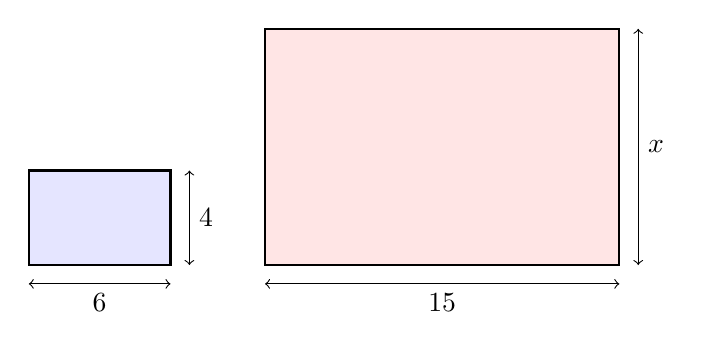
\begin{tikzpicture}[scale=0.6]
  % Smaller
  \draw[thick,fill=blue!10] (0,0) rectangle (3,2);
  \draw[<->] (0,-0.4) -- (3,-0.4);
  \node[below] at (1.5,-0.4) {$6$};
  \draw[<->] (3.4,0) -- (3.4,2);
  \node[right] at (3.4,1) {$4$};
  % Larger
  \draw[thick,fill=red!10] (5,0) rectangle (12.5,5);
  \draw[<->] (5,-0.4) -- (12.5,-0.4);
  \node[below] at (8.75,-0.4) {$15$};
  \draw[<->] (12.9,0) -- (12.9,5);
  \node[right] at (12.9,2.5) {$x$};
\end{tikzpicture}
\end{center}
\end{questionText}
\choiceA{$8$}
\choiceB{$10$}
\choiceC{$12$}
\choiceD{$13$}
\correctAnswer{B}
\explanation{Scale factor: $\frac{15}{6} = 2.5$. $x = 4 \times 2.5 = 10$.}
\end{practiceQuestion}

\begin{practiceQuestion}{6-8-q27}{gmc}
\begin{questionText}
The diagram shows two similar triangles. Find the missing side length $n$.

\begin{center}
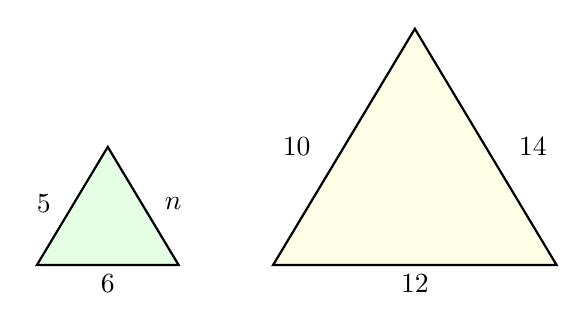
\begin{tikzpicture}[scale=0.6]
  % Small triangle
  \draw[thick,fill=green!10] (0,0) -- (3,0) -- (1.5,2.5) -- cycle;
  \node[below] at (1.5,0) {$6$};
  \node[left] at (0.5,1.3) {$5$};
  \node[right] at (2.5,1.3) {$n$};
  % Large triangle
  \draw[thick,fill=yellow!10] (5,0) -- (11,0) -- (8,5) -- cycle;
  \node[below] at (8,0) {$12$};
  \node[left] at (6,2.5) {$10$};
  \node[right] at (10,2.5) {$14$};
\end{tikzpicture}
\end{center}
\end{questionText}
\choiceA{$4$}
\choiceB{$7$}
\choiceC{$8$}
\choiceD{$9$}
\correctAnswer{B}
\explanation{Scale factor: $\frac{6}{12} = 0.5$ (or $\frac{5}{10} = 0.5$). $n = 14 \times 0.5 = 7$.}
\end{practiceQuestion}

\begin{practiceQuestion}{6-8-q28}{gmc}
\begin{questionText}
The diagram below shows a person and a flagpole casting shadows at the same time. What is the height of the flagpole?

\begin{center}
\begin{tikzpicture}[scale=0.35]
  % Person
  \draw[thick] (0,0) -- (0,4);
  \draw[thick] (0,0) -- (3,0);
  \draw[dashed] (0,4) -- (3,0);
  \node[left] at (0,2) {$4$ ft};
  \node[below] at (1.5,0) {$3$ ft};
  % Flagpole
  \draw[thick] (6,0) -- (6,12);
  \draw[thick] (6,0) -- (15,0);
  \draw[dashed] (6,12) -- (15,0);
  \node[left] at (6,6) {$h$};
  \node[below] at (10.5,0) {$9$ ft};
  % Ground
  \draw[thick] (-1,0) -- (16,0);
\end{tikzpicture}
\end{center}
\end{questionText}
\choiceA{$6$ ft}
\choiceB{$12$ ft}
\choiceC{$16$ ft}
\choiceD{$36$ ft}
\correctAnswer{B}
\explanation{$\frac{4}{3} = \frac{h}{9}$. Cross-multiply: $3h = 36$. Divide: $h = 12$ ft.}
\end{practiceQuestion}

\begin{practiceQuestion}{6-8-q29}{gsa}
\begin{questionText}
The two triangles below are similar. Find the missing side lengths $a$ and $b$.

\begin{center}
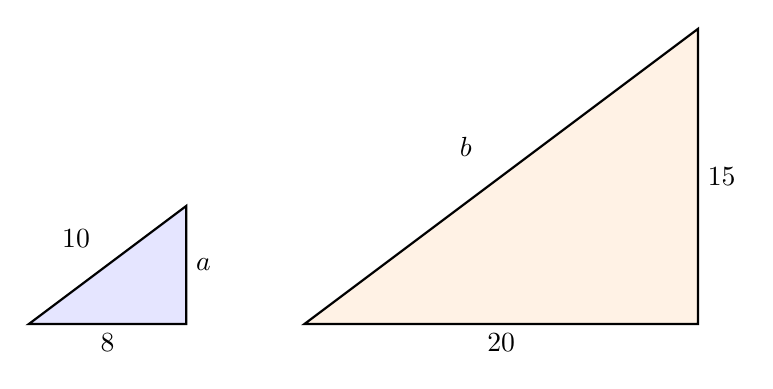
\begin{tikzpicture}[scale=0.5]
  % Small triangle
  \draw[thick,fill=blue!10] (0,0) -- (4,0) -- (4,3) -- cycle;
  \node[below] at (2,0) {$8$};
  \node[right] at (4,1.5) {$a$};
  \node[above left] at (1.8,1.7) {$10$};
  % Large triangle
  \draw[thick,fill=orange!10] (7,0) -- (17,0) -- (17,7.5) -- cycle;
  \node[below] at (12,0) {$20$};
  \node[right] at (17,3.75) {$15$};
  \node[above left] at (11.5,4) {$b$};
\end{tikzpicture}
\end{center}
\end{questionText}
\correctAnswer{$a = 6$, $b = 25$}
\explanation{Scale factor from small to large: $\frac{20}{8} = 2.5$. $a$: from large to small on the right side $= 15 \div 2.5 = 6$. $b$: from small to large on the hypotenuse $= 10 \times 2.5 = 25$.}
\end{practiceQuestion}

\begin{practiceQuestion}{6-8-q30}{gsa}
\begin{questionText}
The grid below shows two similar rectangles. Rectangle $A$ has vertices at $(1, 1)$, $(4, 1)$, $(4, 3)$, $(1, 3)$. Rectangle $B$ has vertices at $(6, 1)$, $(12, 1)$, $(12, 5)$, $(6, 5)$. What is the scale factor from $A$ to $B$?

\begin{center}
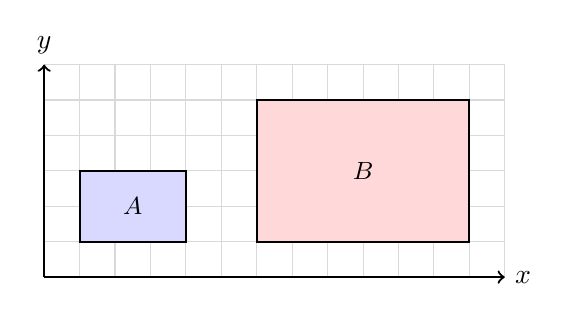
\begin{tikzpicture}[scale=0.45]
  \draw[step=1,gray!30,thin] (0,0) grid (13,6);
  \draw[thick,->] (0,0) -- (13,0) node[right]{$x$};
  \draw[thick,->] (0,0) -- (0,6) node[above]{$y$};
  \draw[thick,fill=blue!15] (1,1) rectangle (4,3);
  \node at (2.5,2) {\small $A$};
  \draw[thick,fill=red!15] (6,1) rectangle (12,5);
  \node at (9,3) {\small $B$};
\end{tikzpicture}
\end{center}
\end{questionText}
\correctAnswer{$2$}
\explanation{Rectangle $A$: width $= 4 - 1 = 3$, height $= 3 - 1 = 2$. Rectangle $B$: width $= 12 - 6 = 6$, height $= 5 - 1 = 4$. Scale factor: $\frac{6}{3} = 2$ (or $\frac{4}{2} = 2$).}
\end{practiceQuestion}
